\begin{frame}{Transactional Memory Variants}
    \onslide<1-> {Most Transactional Memory implementations make use of hardware-assist and are mostly implemented in software.\\}
    \vspace*{0.5cm}
    \onslide<2-> {In this thesis, we focus on Software Transactional Memory introduced by Shavit and Touitou in 1996 [2]\\}
    \vspace*{0.5cm}
    \onslide<3-> {Two main approaches: \textit{non-blocking} and \textit{blocking} STM}
\end{frame}

\begin{frame}{Non-Blocking STM}
    \onslide<1->{Early STM implementations were \textit{non-blocking}.}
    \vspace{0.3cm}
    \onslide<2->{\begin{block}{Definition}
    An algorithm is \textbf{non-blocking} if the delay of one thread does not stop others from making progress.
    \end{block}}
    \vspace{0.3cm}
    \onslide<3->{Non-blocking algorithms utilise lock-free primitives to achieve synchronisation.}
\end{frame}

\begin{frame}{Blocking STM}
\onslide<1->{\begin{itemize}
    \item In 2006, Robert Ennals suggested [3] that the non-blocking property is detrimental to performance.
    \item Following that, attention shifted to \textit{blocking} STM implementations.
\end{itemize}}

\onslide<2->{\begin{block}{Definition}
    An algorithm is \textbf{blocking} if the delay of one thread prevents others from progressing.
    \end{block}
}
    \vspace{0.3cm}
    \onslide<3->{Blocking algorithms utilise locks to achieve synchronisation.}
\end{frame}

\begin{frame}{Blocking STM}
\onslide<1->{\begin{itemize}
    \item Blocking (lock-based) STM implementations lock transactional objects when they wish to modify them
    \item There are two main approaches on how to do that:
\end{itemize}}

\onslide<2->{\begin{block}{Definition}
    \textbf{Encounter-order} transactions lock object as they are encountered.
    \end{block}
}

\onslide<3->{\begin{block}{Definition}
    \textbf{Commit-time} transactions lock object only at commit time, and make tentative changes to memory before that.
    \end{block}
}

\end{frame}

\begin{frame}{Transactional Programming: Interface}
\begin{figure}
    \centering
    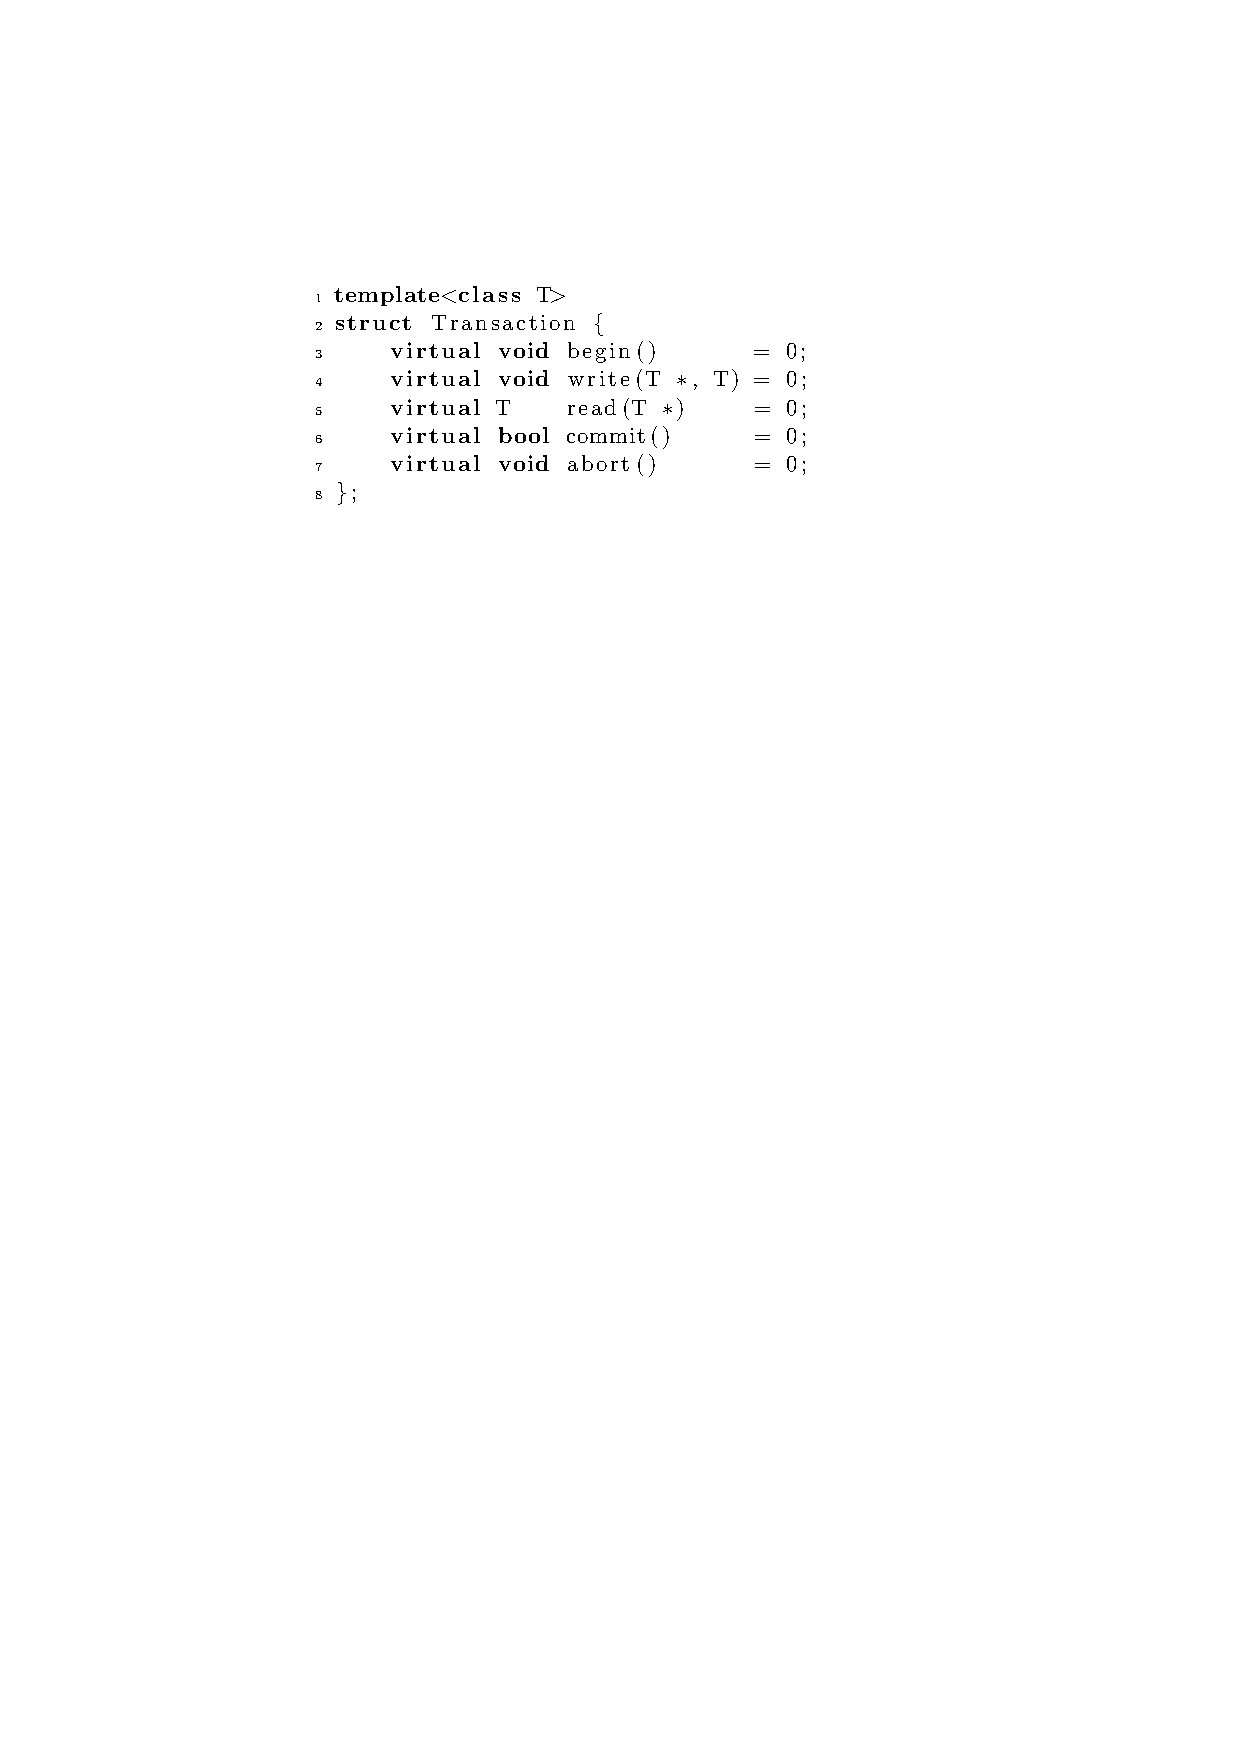
\includegraphics[width=0.7\textwidth]{images/stm-interface.pdf}
\end{figure}
\end{frame}

\begin{frame}{Transactional Programming: Example}
\begin{figure}
    \centering
    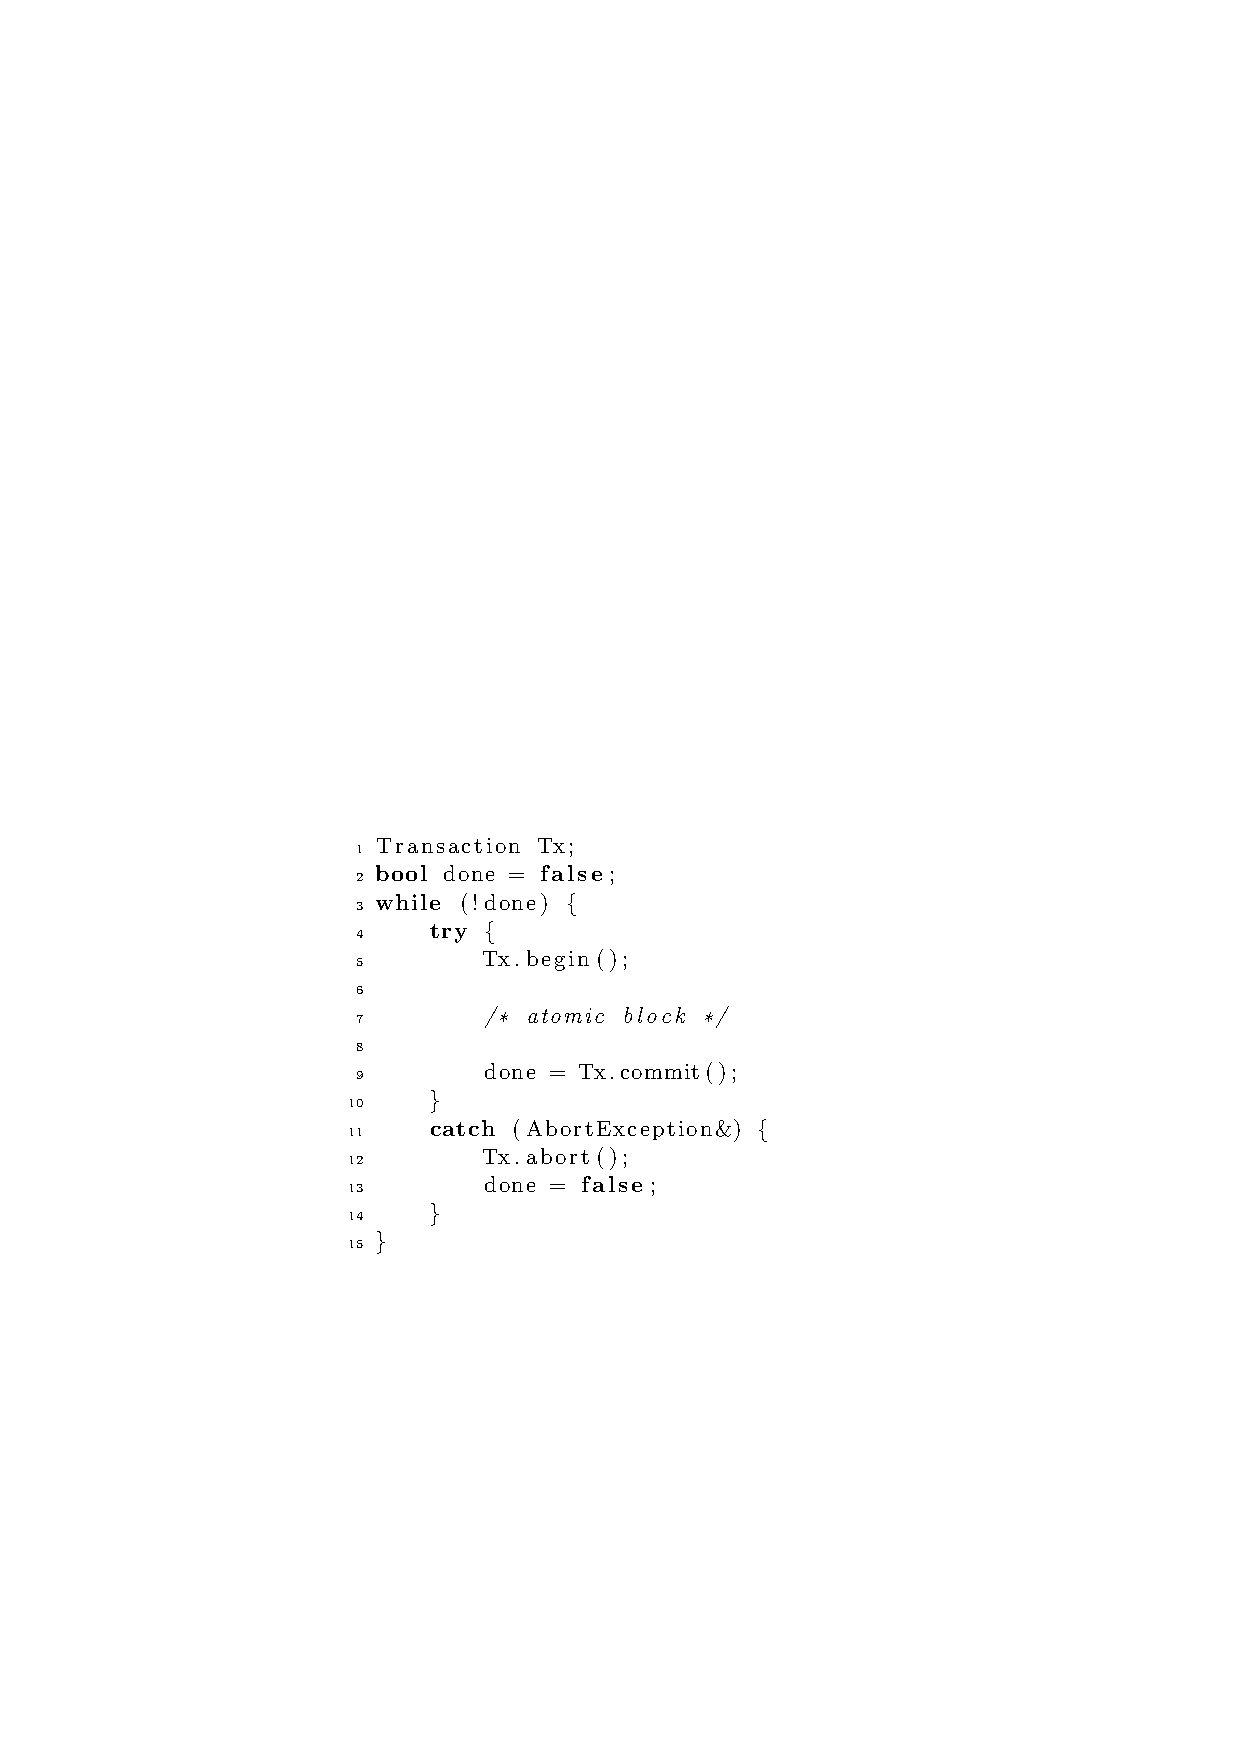
\includegraphics[height=0.7\textheight]{images/stm-example.pdf}
\end{figure}
\end{frame}


